% !TeX root = seminar-02.tex
% !TeX spellcheck = ru-RU
% !TeX encoding = UTF-8 Unicode
% !BIB program = biber
% LTeX: language=ru-RU
% LTeX: enablePickyRules=true
%
% Copyright (c) 2026 Михаил Михайлов
%
% This work is licensed under the Creative Commons Attribution-NonCommercial-ShareAlike 4.0
% International License. To view a copy of this license, visit:
% http://creativecommons.org/licenses/by-nc-sa/4.0/
%
% You are free to:
%   Share - copy and redistribute the material in any medium or format
%   Adapt - remix, transform, and build upon the material
%
% Under the following terms:
%   Attribution - You must give appropriate credit, provide a link to the license,
%                 and indicate if changes were made.
%   NonCommercial - You may not use the material for commercial purposes.
%   ShareAlike - If you remix, transform, or build upon the material, you must
%                distribute your contributions under the same license as the original.
%
% See the LICENSE file in the repository root for full license text.

\documentclass[seminar, recordsfile={../records.lua}]{practice}

\renewcommand{\SeminarName}{Немного кодирования}
\renewcommand{\SeminarDate}{23 января 2025}

\xsimsetup{
	solution/print = true
}

\begin{document}
\subsection*{Алгоритм Шеннона}
\begin{enumerate}[compact]
    \item Упорядочить символы $a_1, a_2, \dots, a_n$ по \emph{возрастанию} длин кодов: $\ell_1 \leq \ldots \leq \ell_n$.
    \item Для символа $a_i$ вычислить:
        \[
		  r_i = \sum_{k=1}^{i - 1} 2^{-\ell_1}, \quad r_1 = 0.
        \]
	\item Взять первые $l_i$ знаков после запятой в двоичном представлении $r_i$. Это и будет кодом $C_i^{\mathrm{S}}$ символа $a_i$.
\end{enumerate}

\begin{exercise}
  Докажите что алгоритм Шеннона всегда строит беспрефиксный код, если длины $\ell_1, \ldots, \ell_n$ удовлетворяют неравенству Крафта.
\end{exercise}
\begin{solution}
Пусть даны длины кодовых слов $l_1 \leq l_2 \leq \ldots \leq l_n$, удовлетворяющие неравенству Крафта. Рассмотрим алгоритм Шеннона. Код строится так: для символа $a_i$ берётся двоичная запись числа $r_i = \sum_{k=1}^{i-1} 2^{-l_k}$ (где $r_1=0$) и в качестве кодового слова используется первые $l_i$ бит после запятой.

Предположим, что код не является беспрефиксным. Тогда существуют индексы $i < j$ такие, что слово $C_i^{\mathrm{S}}$ является префиксом слова $C_j^{\mathrm{S}}$. По построению $C_i^{\mathrm{S}}$ --- это первые $l_i$ бит числа $r_i$, а $C_j^{\mathrm{S}}$ --- первые $l_j$ бит числа $r_j$. Поскольку $l_i \leq l_j$, то из того, что $C_i^{\mathrm{S}}$ --- префикс $C_j^{\mathrm{S}}$, следует, что двоичные представления $r_i$ и $r_j$ совпадают в первых $l_i$ битах после запятой.

Заметим, что $r_j = r_i + \sum_{k=i}^{j-1} 2^{-l_k} \geq r_i + 2^{-l_i}$, так как в сумме присутствует слагаемое $2^{-l_i}$. Но если два числа отличаются не менее чем на $2^{-l_i}$, то их двоичные представления после запятой должны различаться хотя бы в одном из первых $l_i$ битов. Это противоречит совпадению первых $l_i$ битов. Следовательно, наше предположение неверно, и код является беспрефиксным.
\end{solution}

\begin{exercise}
  Пусть вероятность символа $a_i$ равна $p_i$. Докажите что при подходящем выборе $l_i$, средняя длина кода Шеннона $L(C^{\mathrm{S}})$ будет удовлетворять неравенству:
  \[
	  L_{S} \leq \mathrm{H}_2(p_1, \ldots p_n) + 1
  \]
  Код должен быть беспрефиксным.
\end{exercise}
\begin{solution}
Выберем длины кодовых слов $l_i = \lceil -\log_2 p_i \rceil$. Тогда $-\log_2 p_i \leq l_i < -\log_2 p_i + 1$. Проверим условие Крафта:
\[
\	\sum_{i=1}^n 2^{-l_i} \leq \sum_{i=1}^n 2^{\log_2 p_i} = \sum_{i=1}^n p_i = 1.
\]
Следовательно, для этих длин существует беспрефиксный код (по лемме Крафта, а также по предыдущему упражнению, алгоритм Шеннона его построит). Оценим среднюю длину этого кода:
\[
	L_S = \sum_{i=1}^n p_i l_i < \sum_{i=1}^n p_i (-\log_2 p_i + 1) = \mathrm{H}_2(p_1,\dots,p_n) + 1.
\]
Таким образом, для такого выбора $l_i$ код Шеннона удовлетворяет требуемому неравенству.
\end{solution}

\subsection*{Алгоритм Фано}
\begin{enumerate}[compact]
    \item Упорядочить символы по невозрастанию вероятностей.
    \item Разделить множество символов на две части, сумма вероятностей в которых максимально близка друг к другу.
    \item Всем символам в левой части присвоить в начало кода 0, в правой --- 1.
    \item Повторять шаги 2-3 для каждой из частей, пока в части не останется один символ.
\end{enumerate}

\begin{exercise}
  Докажите, что алгоритм Фано всегда строит беспрефиксный код.
\end{exercise}
\begin{solution}
	Алгоритм Фано строит дерево кодирования рекурсивным разбиением множества символов на две части. На каждом шаге каждому символу в одной части добавляется к префиксу 0, а в другой --- 1. Таким образом, код каждого символа соответствует пути от корня дерева к листу. Поскольку разбиение производится до тех пор, пока в каждой части не останется ровно один символ, ни один код не может быть префиксом другого, так как это означало бы, что один символ находится во внутреннем узле дерева, а не в листе. Следовательно, код является беспрефиксным.
\end{solution}

\subsection*{Алгоритм Хаффмана}
\begin{enumerate}[compact]
    \item Создать узлы для каждого символа с его вероятностью. Поместить все узлы в приоритетную очередь минимальная вероятность --- высший приоритет).
    \item Пока в очереди больше одного узла:
	\begin{enumerate}[noitemsep, topsep=0pt, parsep=0pt]
        \item Извлечь два узла с \emph{наименьшими} вероятностями.
        \item Создать новый \emph{внутренний} узел, вероятностью которого будет сумма вероятностей извлеченных узлов.
        \item Сделать извлеченные узлы дочерними для нового (любому присвоить 0, другому --- 1).
        \item Поместить новый узел в очередь.
    \end{enumerate}
    \item Оставшийся узел --- корень дерева. Код символа --- путь от корня к листу (0/1 на каждом ребре).
\end{enumerate}

\begin{exercise}
  Докажите, что алгоритм Хаффмана всегда строит беспрефиксный код.
\end{exercise}
\begin{solution}
  Доказательство беспрефиксности повторяет доказательство беспрефиксности кода Фано mutatis mutandis.
\end{solution}
\subsection*{Кодируем...}
\begin{exercise}
Для алфавита $\set{A, B, C, D}$ с вероятностями $\P(A)=0.45$, $\P(B)=0.25$, $\P(C)=0.2$, $\P(D)=0.1$ выполните:
\begin{enumerate}[compact]
    \item Постройте код Шеннона. Вычислите среднюю длину $L_{\text{S}}$.
    \item Постройте код Фано. Вычислите среднюю длину $L_{\text{F}}$.
    \item Постройте код Хаффмана. Вычислите среднюю длину $L_{\text{H}}$.
	\item Вычислите энтропию источника $\mathrm{H}_2(X) = -\sum p_i \log_2 p_i$.
    \item Сравните избыточности кодов: $R = L_{\text{code}} - H(X)$.
\end{enumerate}
\end{exercise}

\begin{solution}
Дано: $\P(A)=0.45$, $\P(B)=0.25$, $\P(C)=0.2$, $\P(D)=0.1$.

\noindent 1. \textbf{Код Шеннона.} 
Вычислим длины: $l_i = \lceil -\log_2 p_i \rceil$.
\begin{align*}
-\log_2 0.45 &\approx 1.152, \quad l_A = 2; \\
-\log_2 0.25 &= 2.000, \quad l_B = 2; \\
-\log_2 0.2 &\approx 2.322, \quad l_C = 3; \\
-\log_2 0.1 &\approx 3.322, \quad l_D = 4.
\end{align*}
Символы уже упорядочены по возрастанию длин. Вычислим $r_i$:
\begin{align*}
r_A &= 0 = 0.0000_2, \quad \text{код: } 00; \\
r_B &= 2^{-2}=0.25=0.0100_2, \quad \text{код: } 01; \\
r_C &= 2^{-2}+2^{-2}=0.5=0.1000_2, \quad \text{код: } 100; \\
r_D &= 2^{-2}+2^{-2}+2^{-3}=0.5+0.125=0.625=0.1010_2, \quad \text{код: } 1010.
\end{align*}
\noindent Средняя длина: $L_S = 0.45\cdot2 + 0.25\cdot2 + 0.2\cdot3 + 0.1\cdot4 = 0.9+0.5+0.6+0.4 = 2.4$.

\noindent 2. \textbf{Код Фано.}
Алгоритм строит дерево сверху вниз. Графически процесс можно изобразить так:
\begin{center}
\begin{tikzpicture}[
    level distance=15mm,
    level 1/.style={sibling distance=45mm},
    level 2/.style={sibling distance=25mm},
    level 3/.style={sibling distance=15mm},
    every node/.style={draw, circle, minimum size=8mm, inner sep=1pt}
]
% Корень
\node {$\{ABCD\}_{1.0}$}
% Уровень 1
child {
    node {$\{AD\}_{0.55}$}
	child {
		node {$\underset{f(A) = 00}{\{A\}_{0.45}}$}
        edge from parent node[left, yshift=2, xshift=5, draw=none] {0}
	}
	child {
		node {$\underset{f(D) = 01}{\{D\}_{0.1}}$}
        edge from parent node[right, yshift=2, xshift=-5, draw=none] {1}
	}
    edge from parent node[above, yshift=2, draw=none] {0}
}
child {
    node {$\{BC\}_{0.45}$}
    % Уровень 2
    child {
		node {$\underset{f(B) = 10}{\{B\}_{0.25}}$}
        edge from parent node[left, yshift=2, xshift=5, draw=none] {0}
    }
    child {
		node {$\underset{f(D) = 11}{\{C\}_{0.2}}$}
        edge from parent node[right, yshift=2, xshift=-5, draw=none] {1}
    }
    edge from parent node[above, yshift=2, draw=none] {1}
};
\end{tikzpicture}
\end{center}
\noindent Средняя длина: $L_{F} = 2$.

\newpage
\noindent 3. \textbf{Код Хаффмана.}
Имеем:
\begin{center}
\begin{tikzpicture}[
    level distance=15mm,
    level 1/.style={sibling distance=25mm},
    level 2/.style={sibling distance=15mm},
    level 3/.style={sibling distance=10mm},
    every node/.style={draw, circle, minimum size=8mm, inner sep=1pt}
]
\node {$R_{1.0}$}
child {
    node {$A_{0.45}$}
    edge from parent node[left, draw=none] {0}
}
child {
    node {$X_{0.55}$}
    child {
        node {$B_{0.25}$}
        edge from parent node[left, draw=none] {0}
    }
    child {
        node {$X_{0.3}$}
        child {
            node {$C_{0.2}$}
            edge from parent node[left, draw=none] {0}
        }
        child {
            node {$D_{0.1}$}
            edge from parent node[right, draw=none] {1}
        }
        edge from parent node[right, draw=none] {1}
    }
    edge from parent node[right, draw=none] {1}
};
% Подписи кодов
\node[draw=none, anchor=west] at (6, 0.0) {Коды:};
\node[draw=none, anchor=west] at (6, -0.5) {$A: 0$ (путь: 0)};
\node[draw=none, anchor=west] at (6, -1.0) {$B: 10$ (путь: 1$\to$0)};
\node[draw=none, anchor=west] at (6, -1.5) {$C: 110$ (путь: 1$\to$1$\to$0)};
\node[draw=none, anchor=west] at (6, -2.0) {$D: 111$ (путь: 1$\to$1$\to$1)};
\end{tikzpicture}
\end{center}

Средняя длина: $L_H = 1.85$.

\noindent \textbf{Энтропия и избыточности.} Пусть $X$ обозначает случайный символ. Имеем:
\begin{align*}
\mathrm{H}_2(X) &= -\sum p_i \log_2 p_i \\
&\approx 0.45\cdot1.152 + 0.25\cdot2 + 0.2\cdot2.322 + 0.1\cdot3.322 \\
&\approx 0.5184 + 0.5 + 0.4644 + 0.3322 = 1.815.
\end{align*}
Тогда:
\begin{align*}
	R_S &= L_S - \mathrm{H}_2(X) \approx 2.4 - 1.815 = 0.585; \\
	R_{F} &= L_{SF} - \mathrm{H}_2(X) \approx 2 - 1.815 = 0.185; \\
	R_H &= L_H - \mathrm{H}_2(X) \approx 1.85 - 1.815 = 0.035.
\end{align*}
\end{solution}
\end{document}
